\documentclass[a4paper,12pt,oneside]{ujbook}
\usepackage{amsmath,amssymb,ascmac,bm}
%\usepackage[dvips]{graphicx}
\usepackage{subfigure}
\usepackage{longtable}
\usepackage{multirow}
\usepackage{thesis}
\usepackage[dvipdfmx]{graphicx}

\begin{document}

\title{
	<令和元年度専攻科研究論文>\\
	畳み込み辞書学習を用いた\\クラス分類の検討\\ \\
	指導教官: 黒木祥光 教授\\
	機械・電気システム工学専攻 A3519 平川智也
}
\date{}
\maketitle

\tableofcontents

\chapter{はじめに}
近年,畳み込みニューラルネットワーク(CNN)は,パターン・画像認識分野の様々なタスクにおいて強力な手法として知られている.
CNNを画像分類問題に適用する場合,画像とラベルデータを用いて誤差逆伝搬法によってネットワークを学習する.
これに対し,畳み込み辞書学習と呼ばれる手法が提案されている\cite{fast-csc}.
畳み込み辞書学習はフィルタと係数マップへの信号分離の最適化問題として定式化され,ラベルデータを用いずに画像のみからデータ駆動的に特徴を抽出する.
畳み込み辞書学習は最適化ベースの特徴抽出法であるため,制約や目的関数の変更が柔軟にでき,単に特徴抽出だけでなく,画像の超解像度の研究\cite{super-res}などに応用されている.

本研究では畳み込み辞書学習問題における係数マップを特徴とする,錐制約部分空間法を分類問題に適用する.
その際に,係数マップのパワースペクトルを使用することにより,データセット内の各データ間に存在する位置ずれに対する頑健性を高める.
CNNでは,新たなクラスが加わった際に,はじめから再学習する必要があるのに対して,部分空間法では,新たなクラスの張る部分空間を設計すればよいのでコストが低いことなどを考慮し,本研究では部分空間法を基にした分類器を適用する.
具体的には,パワースペクトルは非負値をとるため,特徴群は錐の形状をなすと仮定し,部分空間法に錐制約を課した錐制約部分空間法を適用する.


\chapter{畳み込み辞書学習}
\section{辞書学習問題}
\begin{figure}[htb]
	\centering
	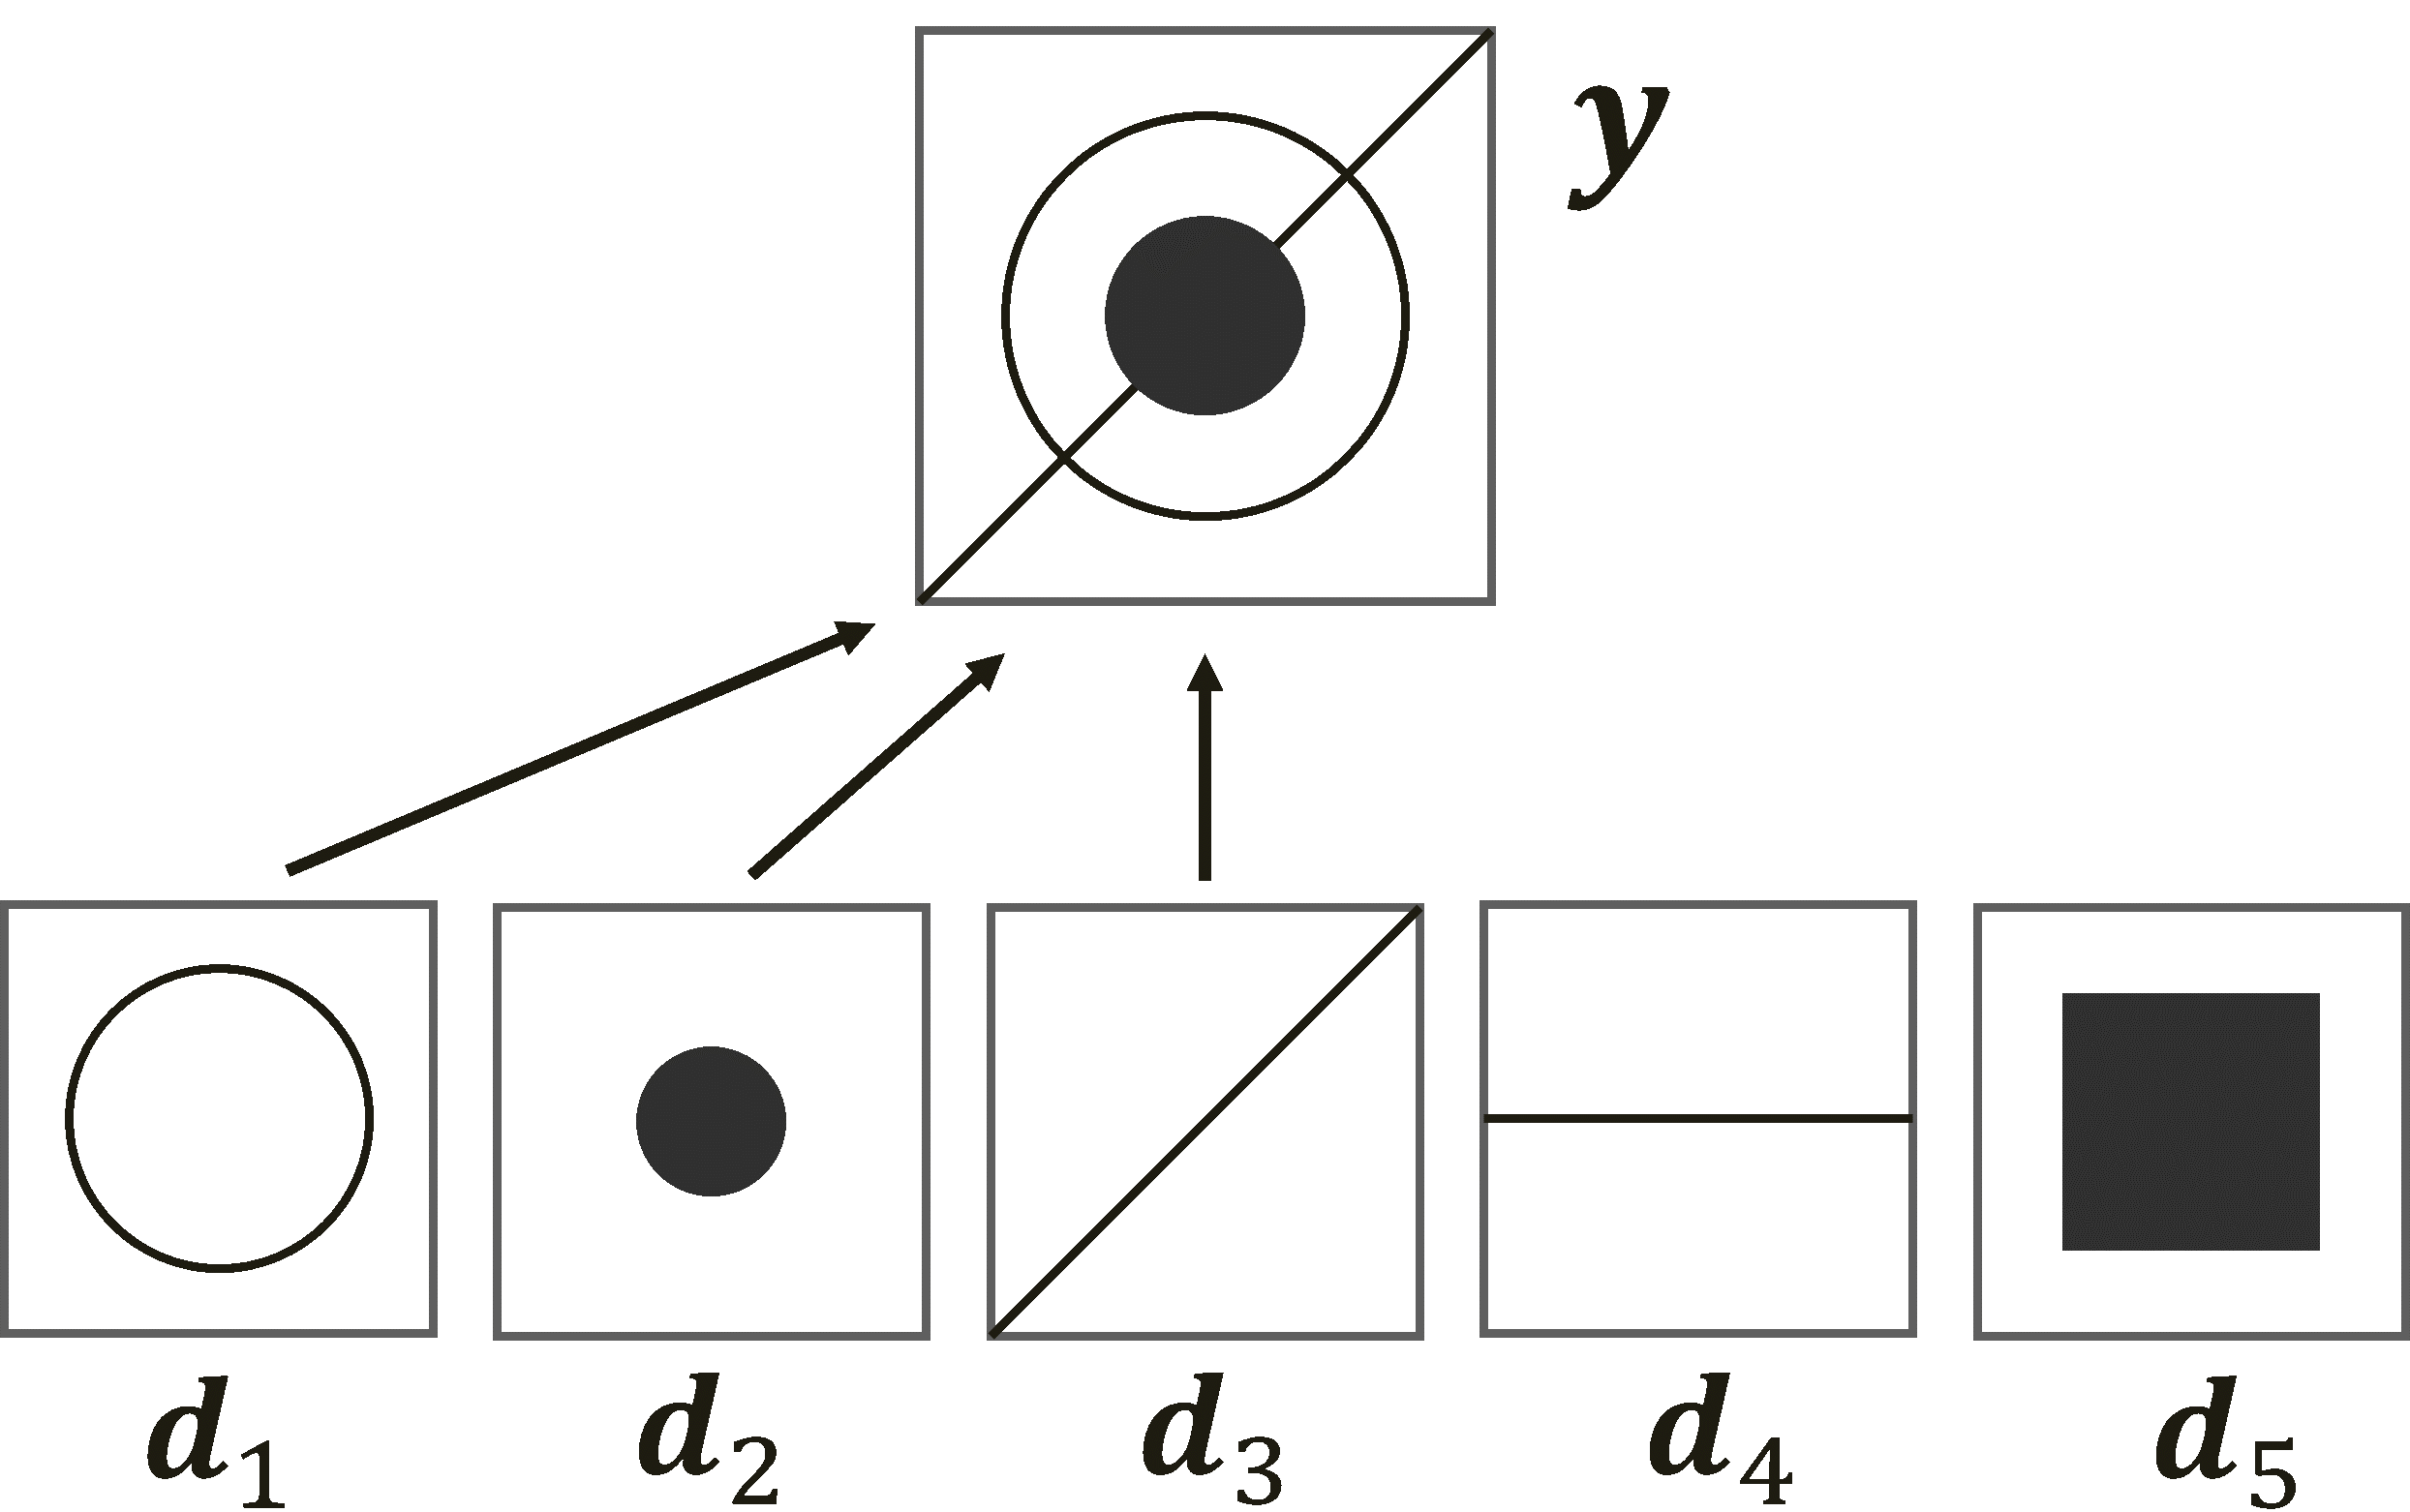
\includegraphics[width=0.7\linewidth]{image/dl}
	\caption{辞書学習のイメージ}
	\label{fig:dl}
\end{figure}

辞書学習問題では,与えられた$d$次元の信号$\bm y\in\mathbb{R}^d$ を,$K$個の辞書基底ベクトル$\bm d_i\in\mathbb{R}^d~(i=1,...,K)$と,疎な係数$\bm x_j\in\mathbb{R}^K$の線形結合で表現する問題であり,以下の最適化問題で記述される.
\begin{equation}
	D_{\text{opt}},\bm x_{\text{opt}}=\arg\min_{D, \bm x}\frac{1}{2}\|\bm y-D\bm x\|_2^2+\lambda\|\bm x\|_1~~~\text{s.t.}~~~\|\bm d_i\|_2\leq 1
	\label{dict-learn}
\end{equation}
ここで,$D=[\bm d_1,...,\bm d_K]$ であり,パラメータ$\lambda$はデータの再現精度と係数の疎性を調節するパラメータである.
問題(\ref{dict-learn})は,2変数の最適化問題であるが一般に$D$の最適化問題(辞書更新),$\bm x$の最適化問題(係数推定)に分割され,それらを繰り返し交互に解くことで解を得る.
画像処理における辞書学習問題の応用では,入力画像を小領域のパッチに分割して処理することが多い.
そのため,パッチ分割によるブロックノイズやエイリアジングが生じることがある.

\section{畳み込み辞書学習問題}
\begin{figure}[htb]
	\centering
	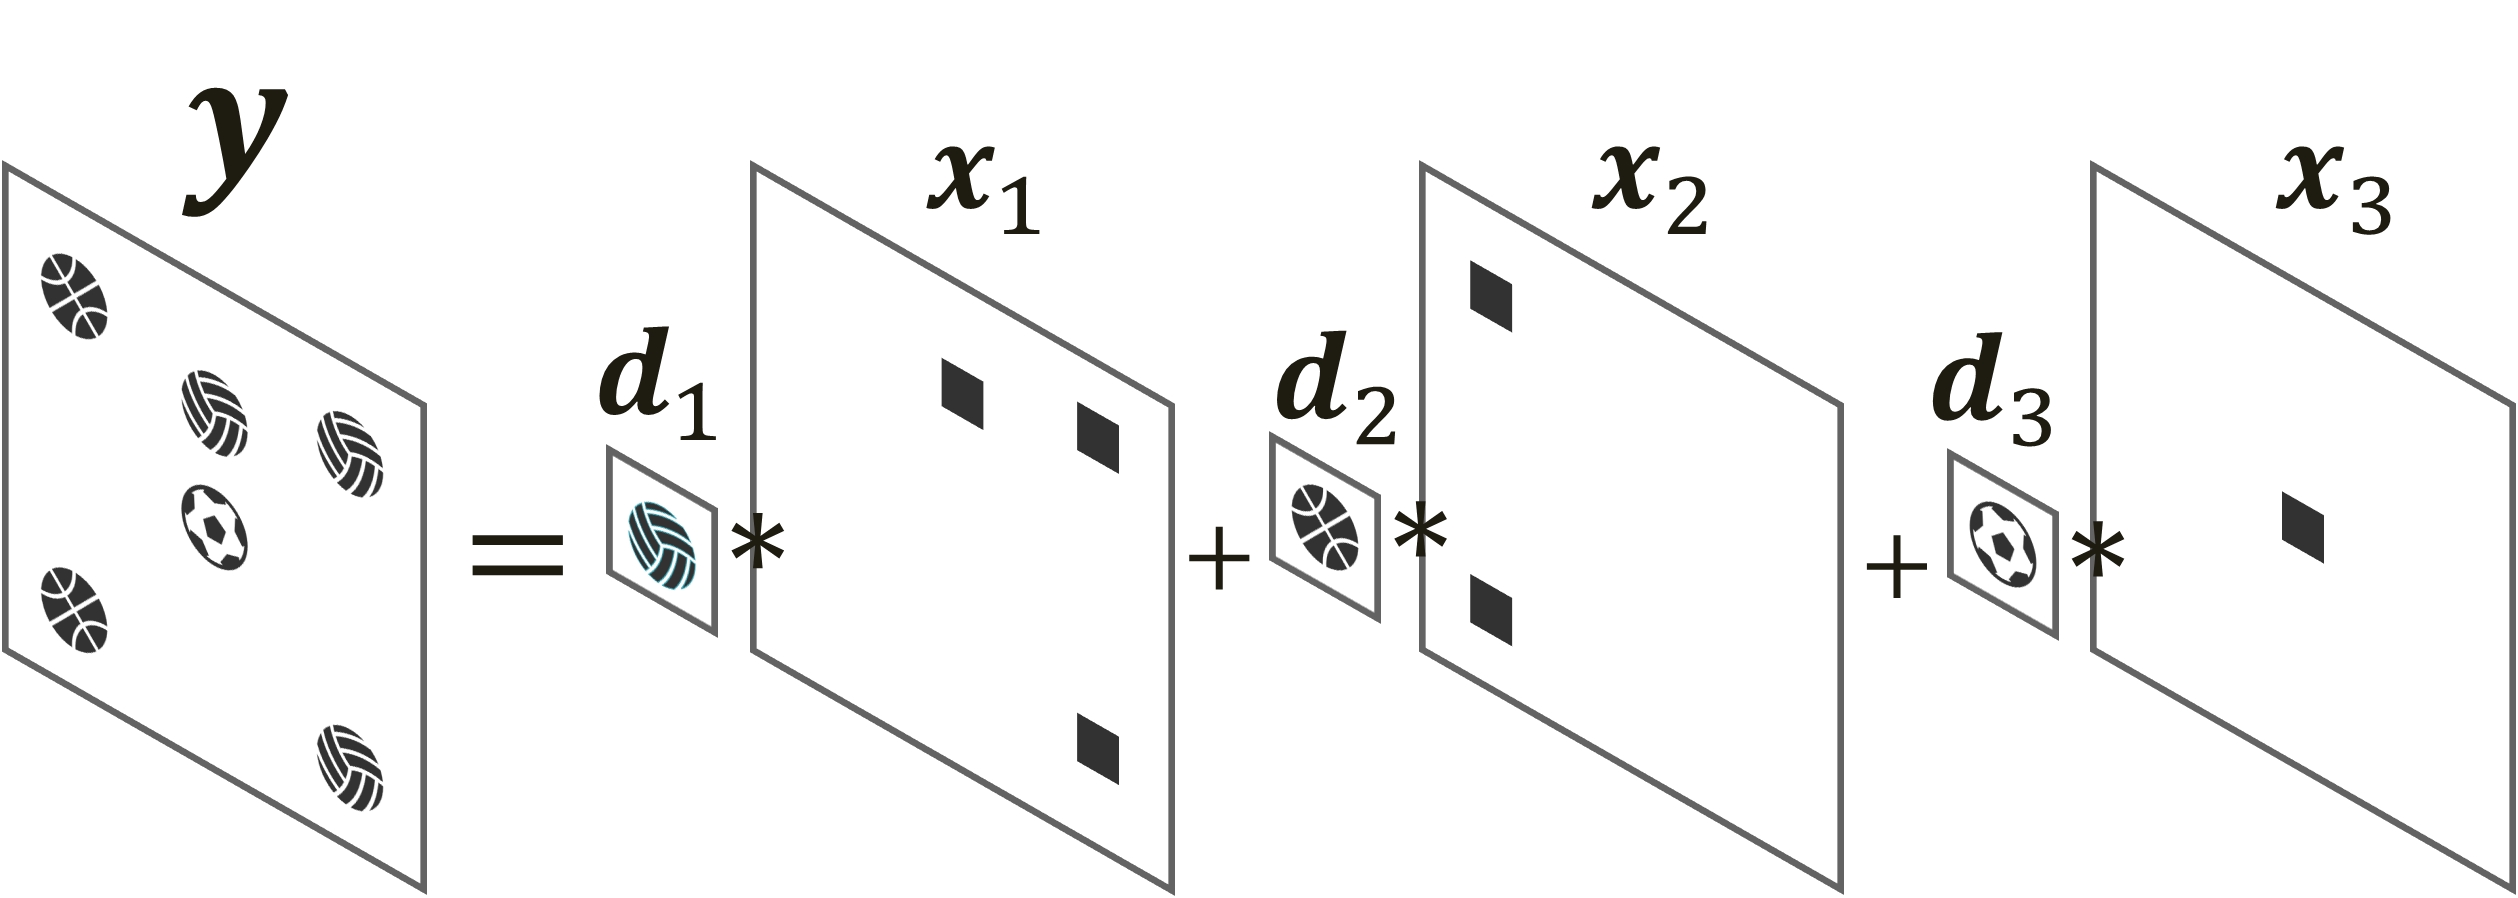
\includegraphics[width=0.7\linewidth]{image/cdl}
	\caption{畳み込み辞書学習のイメージ}
	\label{fig:cdl}
\end{figure}

畳み込み辞書学習では,与えられたサイズが$H\times W$の入力画像$\bm y\in\mathbb{R}^{H\times W}$を,サイズが$h\times w$の$K$個のフィルタ$\bm d_i\in\mathbb{R}^{h\times w}(i=1,...,K)$と,入力画像と同じサイズの$K$個の疎な係数マップの畳み込み和で表現する問題であり,以下の最適化問題で記述される.
\begin{equation}
	D_{\text{opt}},X_{\text{opt}}=\arg\min_{\bm d_i,\bm x_i}\frac{1}{2}\left\|\bm y-\sum_{i=1}^{K}\bm d_i*\bm x_i\right\|_2^2+\lambda\sum_{i=1}^{K}\|\bm x_i\|_1~~\text{s.t.}~~\bm d_i\in C_d,\bm x_i\in C_x
	\label{cdict-learn}
\end{equation}
ここで,$D=[\bm d_1, ..., \bm d_K]\in\mathbb{R}^{h\times w\times K}, X=[\bm x_1,...,\bm x_K]\in\mathbb{R}^{H\times W\times K}$ であり,$*$は巡回畳み込みを示す.
パラメータ$\lambda$はデータの再現精度と係数マップの疎性を調節するパラメータである.
$C_d, C_x$はそれぞれ,フィルタと係数マップに対する凸制約集合で,$D_{\text{opt}},X_{\text{opt}}$は問題の最適値であることを示す.
問題(\ref{cdict-learn})は,2変数の最適化問題であるため,以下に示す各変数についての最適化問題に分割する.
\begin{equation}
	D_{\text{opt}} = \arg\min_{\bm d_i}\frac{1}{2}\left\|\bm y-\sum_{i=1}^{K}\bm d_i*\bm x_i\right\|_2^2~~\text{s.t.}~~\bm d_i\in C_d
	\label{D-update}
\end{equation}
\begin{equation}
	X_{\text{opt}}=\arg\min_{\bm x_i}\frac{1}{2}\left\|\bm y-\sum_{i=1}^{K}\bm d_i*\bm x_i\right\|_2^2+\lambda\sum_{i=1}^{K}\|\bm x_i\|_1~~\text{s.t.}~~\bm x_i\in C_x
\label{x-update}
\end{equation}
問題(\ref{D-update})(\ref{x-update})を,辞書更新および係数推定の問題であり,どちらも凸最適化問題で定式化される.
両問題ともに凸計画問題の反復解法である交互方向乗数法(Alternating Direction Method of Multipliers: ADMM)\cite{admm}によって解かれ,各問題を交互に繰り返し解くことで所望の解を得る.

\chapter{錐制約部分空間法}
\section{錐の定義}
特徴ベクトル空間でサンプルベクトルが張る凸錐は以下で定義される.
\begin{equation}
	C:=\left\{\bm x|\bm x=\sum_{i=1}^{N}c_i\bm \xi_i=\Xi\bm c, \bm c\geq \bm 0\right\}
\end{equation}
ここで$N$は錐の基底ベクトル$\bm \xi_i\in\mathbb{R}^d$の数,$c_i$は非負の結合係数,$\Xi=[\bm \xi_1~\bm \xi_2~...~\bm \xi_N]$,$\bm c={}^t(c_1, c_2,.., c_N)$である.
錐は部分空間における結合係数に非負制約を課したものであり,部分空間と同様にスケール変化・ベクトルの加法に対して閉じた表現となっている.

\section{錐への角度}
錐制約部分空間法では,入力ベクトルと各クラスの錐とのなす角度によって分類を行う.角度$\theta$は入力特徴ベクトル$\bm y$とその錐$C$への正射影ベクトルのなす角度で定義される.
\begin{equation}
	\theta = \arcsin\left(\min_{\bm x\in C}\frac{\|\bm y-\bm x\|}{\|\bm y\|}\right)=\arcsin\left(\frac{1}{\|\bm y\|}\sqrt{\min_{\bm c\geq \bm 0}\|\bm y-\Xi\bm c\|^2}\right)
\end{equation}
ここで$0\leq\theta\leq\frac{\pi}{2}$である.
これは非負値最小二乗法を適用することで得られる.

\section{錐の構成方法}
凸錐の構成方法については様々な手法が提案されている\cite{cone-sub}が,本研究では非負値行列因子分解(Nonnegative Matrix Factrolization:NMF)\cite{nmf}による手法と,特徴ベクトルを包括する凸錐を構成する手法を採用した.
以下に概略を示す.
\subsection{NMFによる錐の構成}
NMFは$n\times m$の非負値行列$V$を$n\times r$の非負値行列$W$と$r\times m$の非負値行列$H$の行列積で表現する手法である.
$V=(v_{ij}),W=(w_{ij}),H=(h_{ij})$とし,$V,W,H$の$j$列目の列ベクトルをそれぞれ$\bm v_j={}^t(v_{1j}, ..., v_{nj}),\bm w_j={}^t(w_{1j}, ..., w_{nj}),\bm h_j={}^t(h_{1j}, ..., h_{rj})$と表すと,$\bm v_j$については
\begin{equation}
	\bm v_j\approx W\bm h_j=h_{1j}\bm w_{1}+h_{2j}\bm w_2+\cdots+h_{rj}\bm w_{r}
\end{equation}
と表され,$V$の列ベクトル$\bm v_j$を$W$の$r$個の列ベクトルの線形結合で近似しており,その結合係数が$\bm h_j$となる.
このため,分解後の行列$W$には錐の基底ベクトルが格納される.

\subsection{包括凸錐の構成}
\begin{figure}[htb]
	\centering
	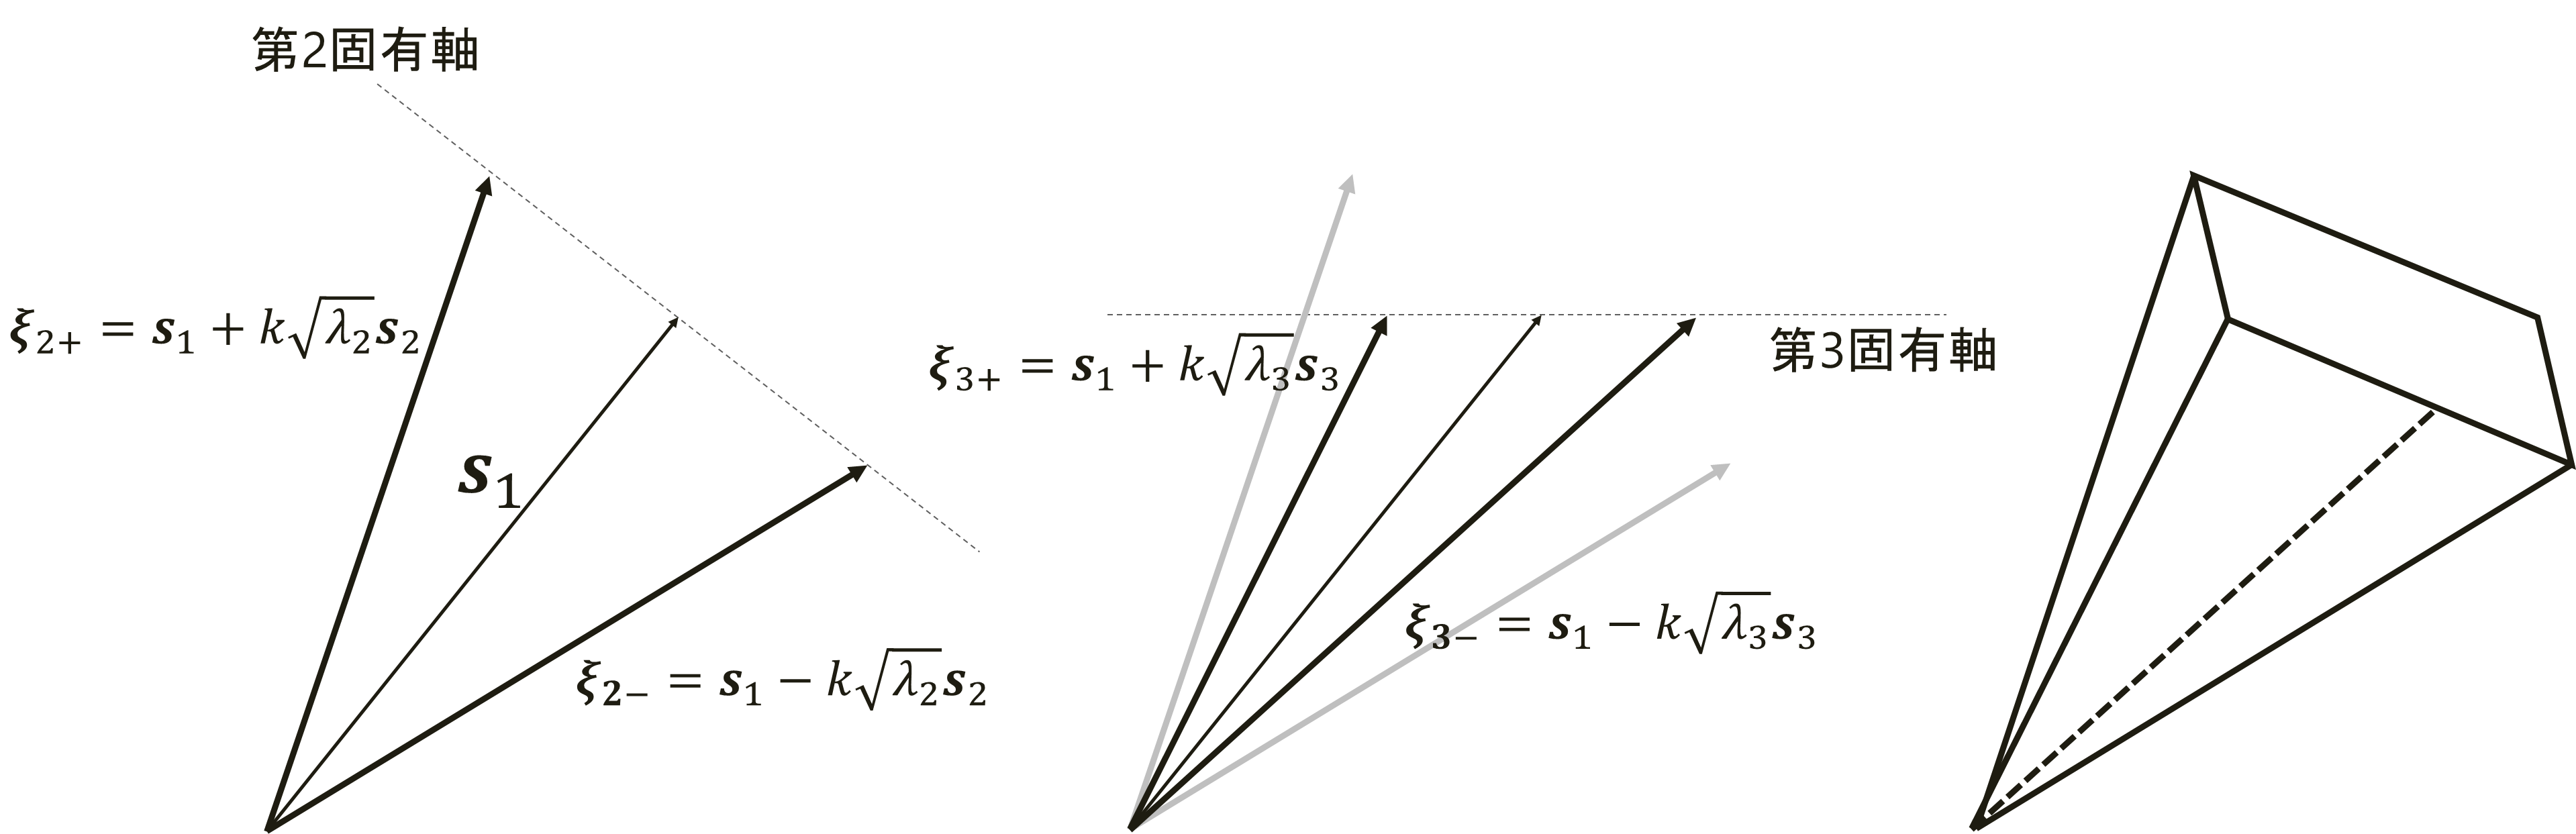
\includegraphics[width=0.7\linewidth]{image/comprehensive_cone}
	\caption{包括凸錐の構成方法(3次元空間での例)}
	\label{fig:comprehensivecone}
\end{figure}

錐のモデルとして\cite{cone-sub}は厳密な凸錐,包括凸錐,円錐を提案しているが,本研究では近似精度と計算量のバランスが良い包括凸錐を扱う.
包括凸錐は特徴ベクトル集合のなす凸錐を少数の基底ベクトルからなる包括的な凸錐で近似する手法である.
先ず,特徴ベクトル$\bm x_i\in\mathbb{R}^d$を単位超球面上に射影する.
\begin{equation}
	\bm z_i=\frac{\bm x_i}{\|\bm x_i\|}
\end{equation}
次に$\bm z_i$の自己相関行列に主成分分析(PCA)を適用する.
これにより得られた固有ベクトルを固有値の大きさに従い降順に並べたとき,第1固有ベクトルは原点からの凸錐の方向(中心),それに直交する第2以降の固有ベクトルは超球面上の特徴ベクトル集合の分布の広がりとなる.
この分布を包括する凸包は第2以降の各固有軸上で分布を包括する(分布の端点などの)2点$(\bm x_L,\bm x_R)$を選ぶことによって構成される.
つまり,各固有軸$(i\geq 2)$に対して次の2つの錐の基底ベクトルが定まる.
\begin{equation}
	\bm \xi_{i-}=\bm s_1+x_L^i\bm s_i=\bm s_1-k\sqrt{\lambda_i}\bm s_i
\end{equation}
\begin{equation}
\bm \xi_{i+}=\bm s_1+x_R^i\bm s_i=\bm s_1+k\sqrt{\lambda_i}\bm s_i
\end{equation}
ここで,$\bm s_i, \lambda_i$はそれぞれ第$i$固有ベクトル,固有値となり,$k$はスケーリングのパラメータである.
第1固有ベクトルが錐の中心ベクトルとなることから,第2以降の固有軸上での分布は原点が中心となり,その分散は固有値$\lambda_i$で与えられる.
ここでは外れ値の影響を考慮し,各軸上で標準偏差の$k$倍の点を選んでいる.

\chapter{提案法}
\begin{figure}[htb]
	\centering
	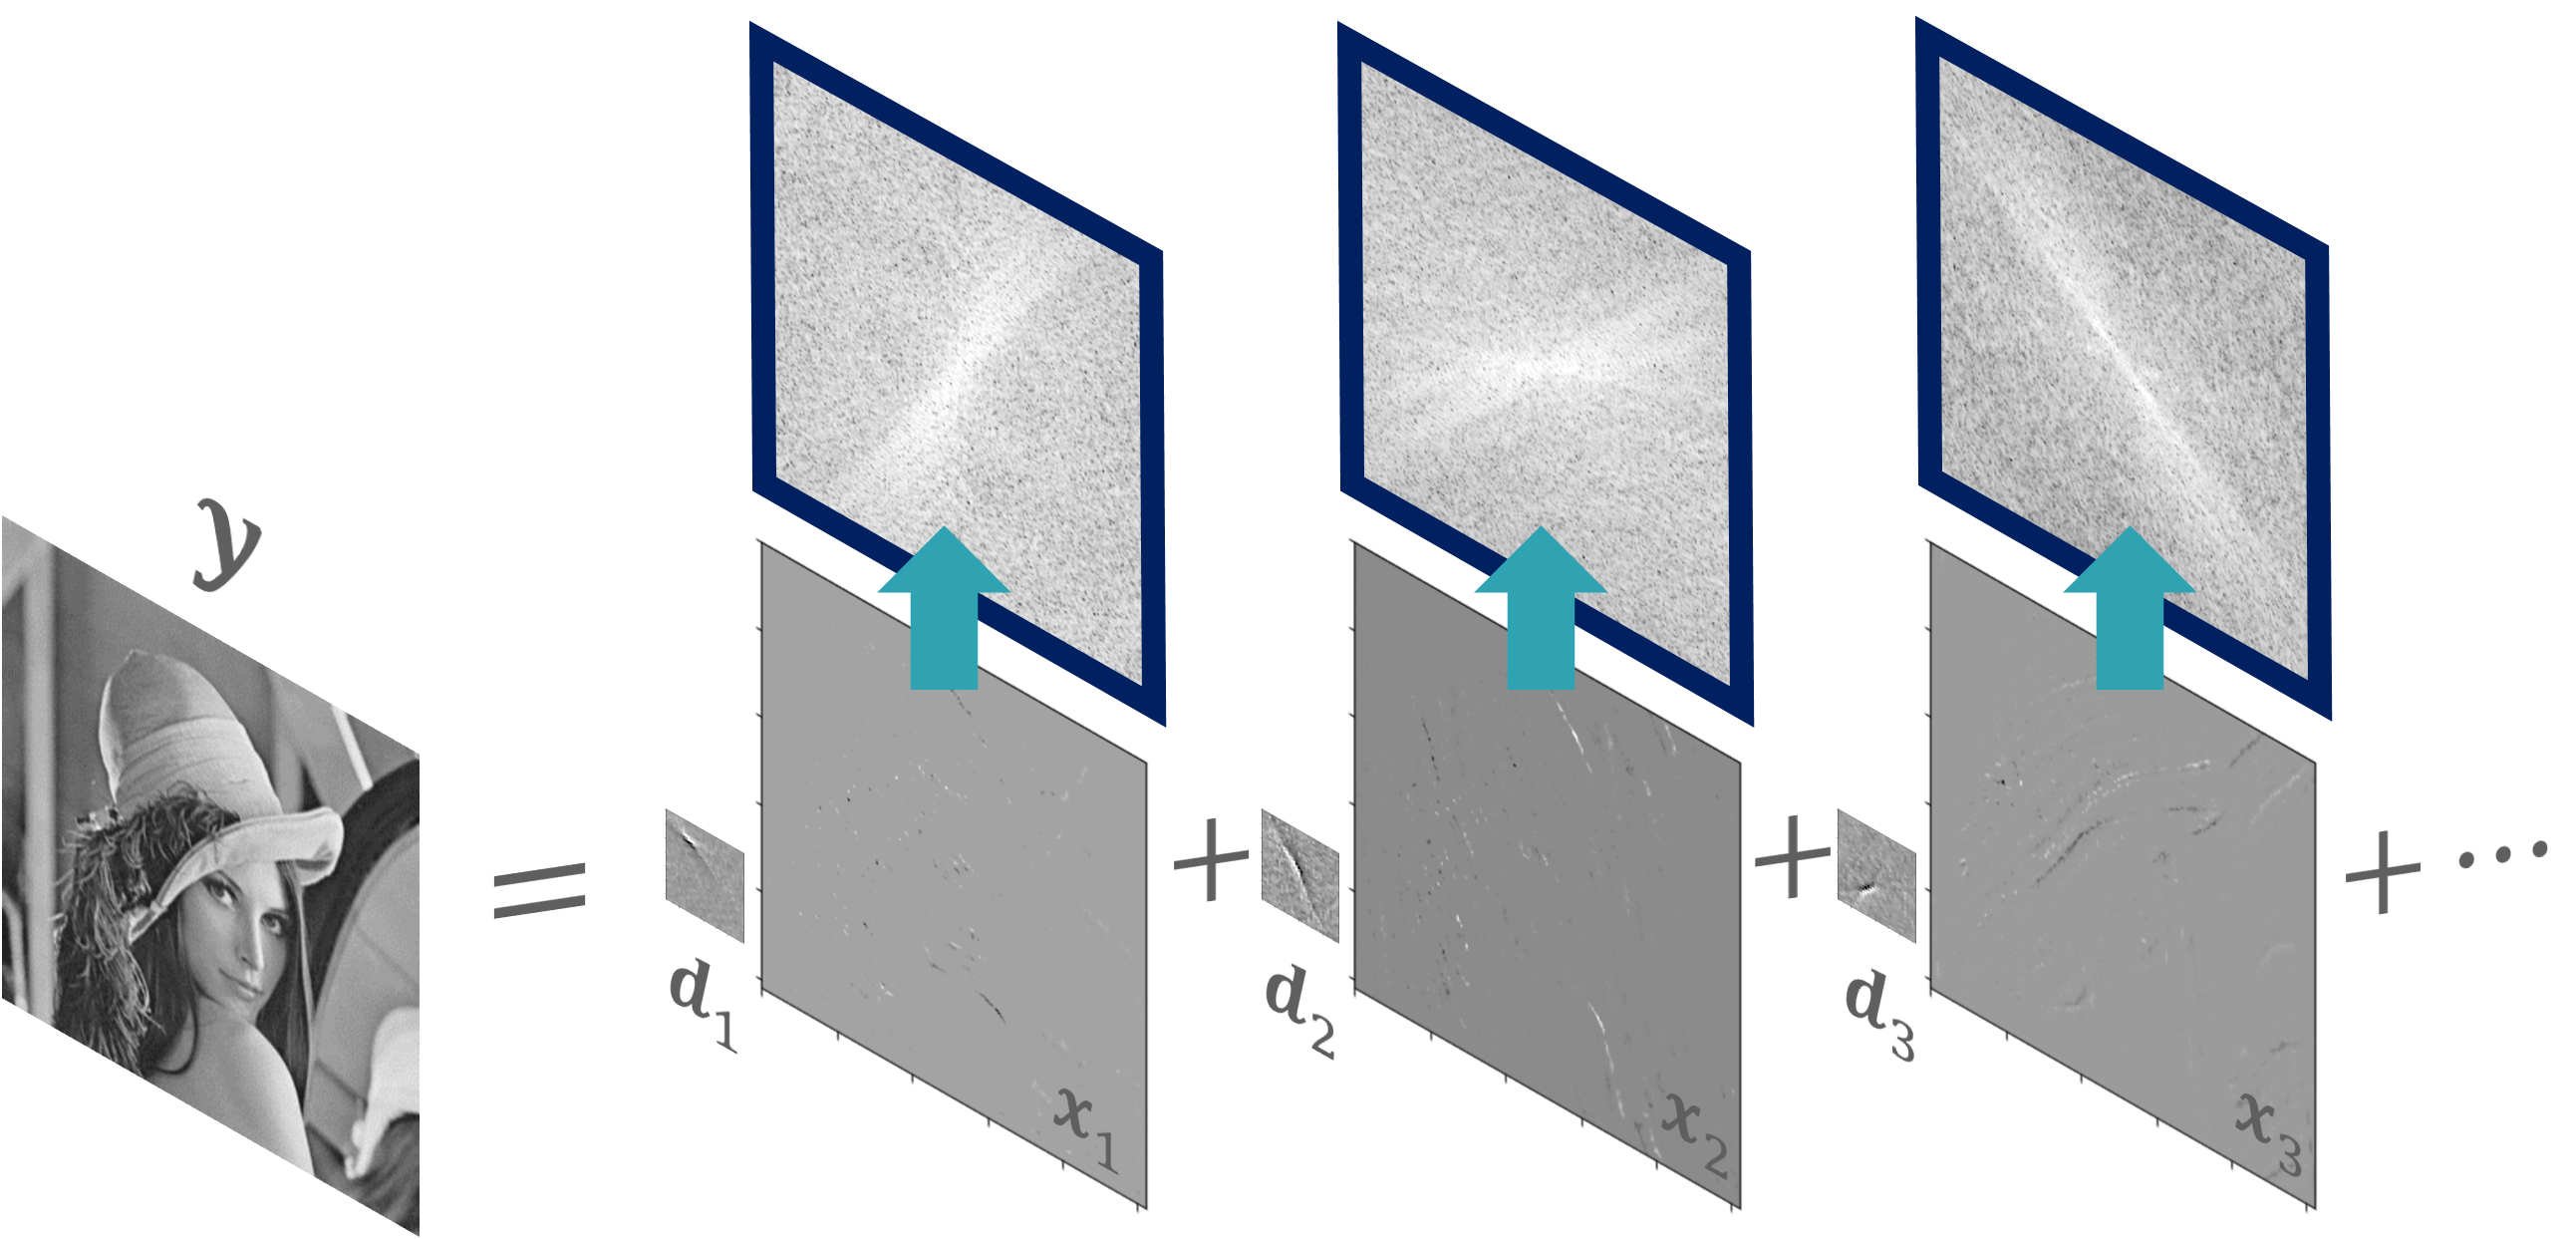
\includegraphics[width=0.7\linewidth]{image/power-spectrum}
	\caption{提案法で使用する特徴(図中の太枠部分)}
	\label{fig:power-spectrum}
\end{figure}

畳み込み辞書学習におけるフィルタは,エッジやテクスチャなどの局所的な特徴をとらえるのに対し,係数マップはフィルタの示す特徴が入力信号のどの部分に顕在しているのかを示す.
したがって,入力信号がシフト変動を受けるとき,係数マップも近しい変動を受けると考えられる.
そこで本研究では,疎な係数マップのパワースペクトル(図\ref{fig:shift})を特徴として用いることで,シフト変動に頑健な特徴を設計する.
パワースペクトルはその信号に含まれる各周波数成分の振幅を示すものである.
これにより,データセット内の各データ間の位置ずれに対して頑健な特徴抽出が可能となる.

\begin{figure}[htb]
	\centering
	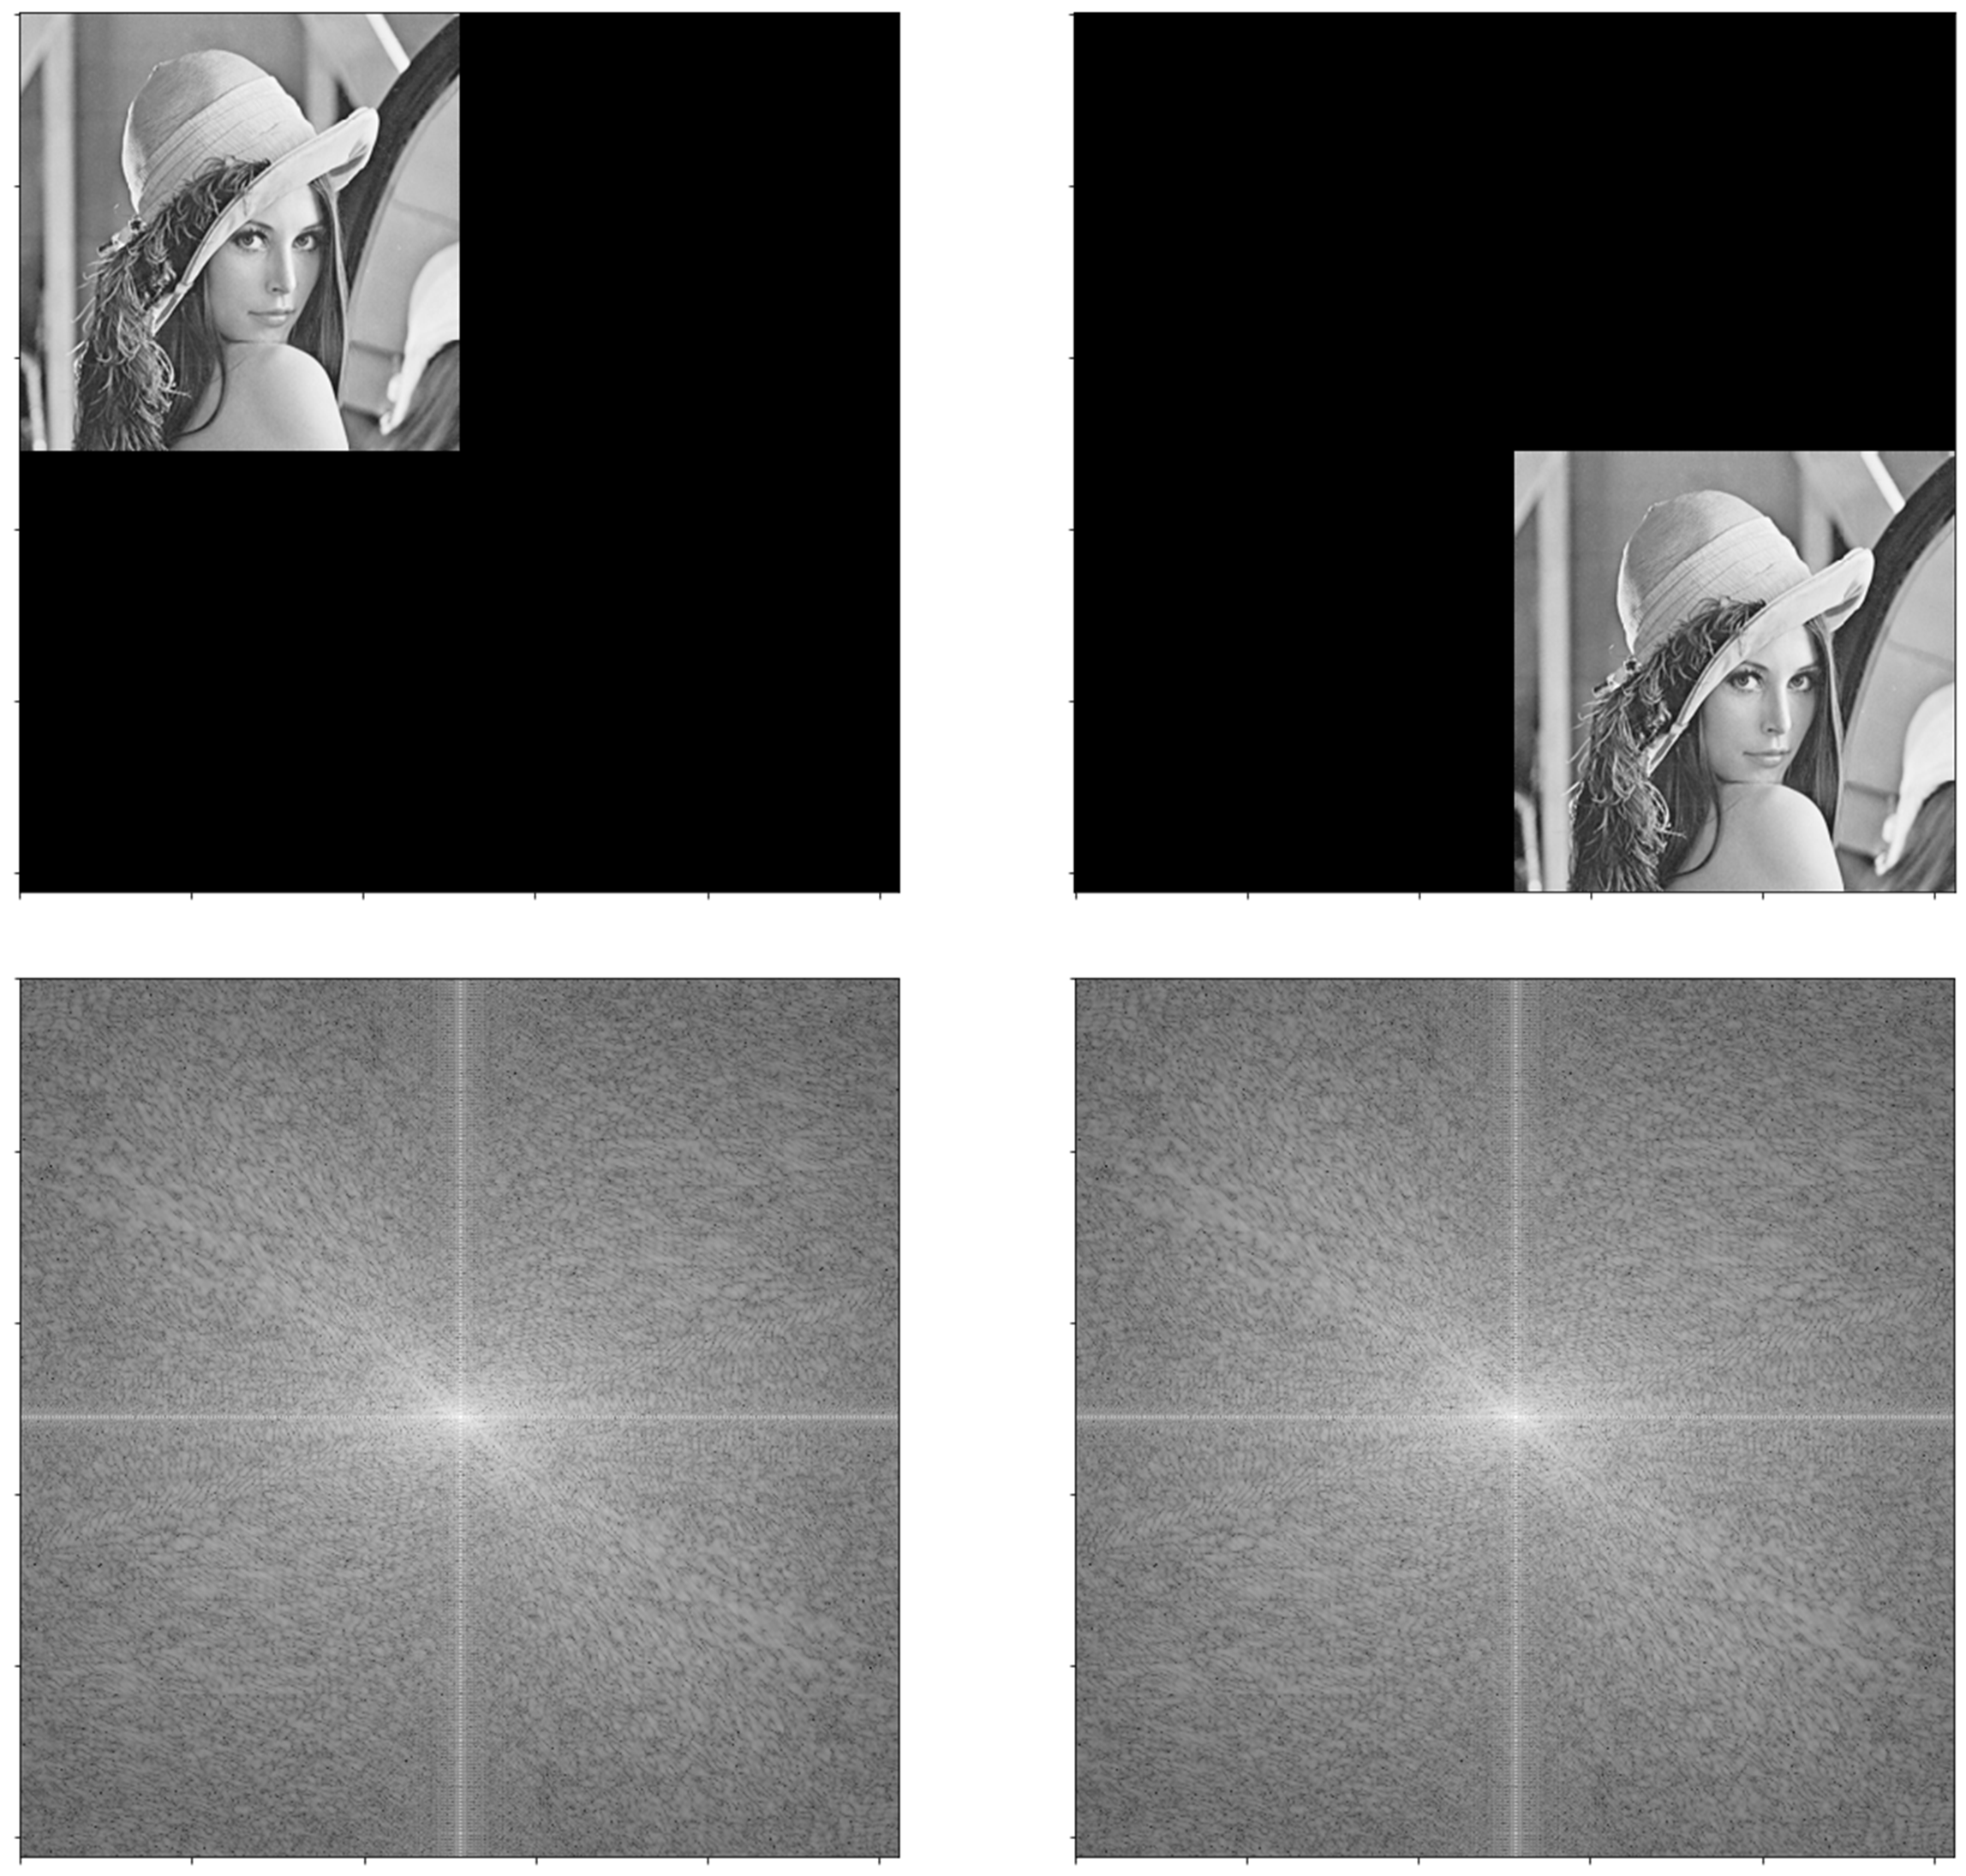
\includegraphics[width=0.7\linewidth]{image/shift}
	\caption{シフト変動させた信号に対するパワースペクトル}
	\label{fig:shift}
\end{figure}

また,本研究ではパワースペクトルの非負値性を利用し,部分空間法ではなく,錐制約を課した部分空間法を分類問題に適用する.

\chapter{実験}
\section{実験}
実験には10クラスの手書き数字文字画像からなるデータセットであるMNISTを使用した.
データセットは$32\times 32$ピクセルの8ビットグレースケール画像からなる.
本実験では,データセットのうち1000枚をテスト用データに割り当てた.
学習用データの画像枚数は100, 200, 300, 400, 500, 1000 と変化させた.
本研究では,パワースペクトルの使用が分類精度にどう影響するか,また錐制約部分空間法は他の分類器と比較してどのような特徴を持つのか,に焦点を当てる.
したがって,分類に使用する特徴は,畳み込み辞書学習における係数マップおよび畳み込み辞書学習における係数マップのパワースペクトルの2種類で比較する.
また,分類器については,NMFで構成された錐での錐制約部分空間法,包括凸錐による錐制約部分空間法に加えて,3層ニューラルネットワーク,Support Vector Machine (SVM)を分類器として使用した.


\begin{figure}[htb]
	\centering
	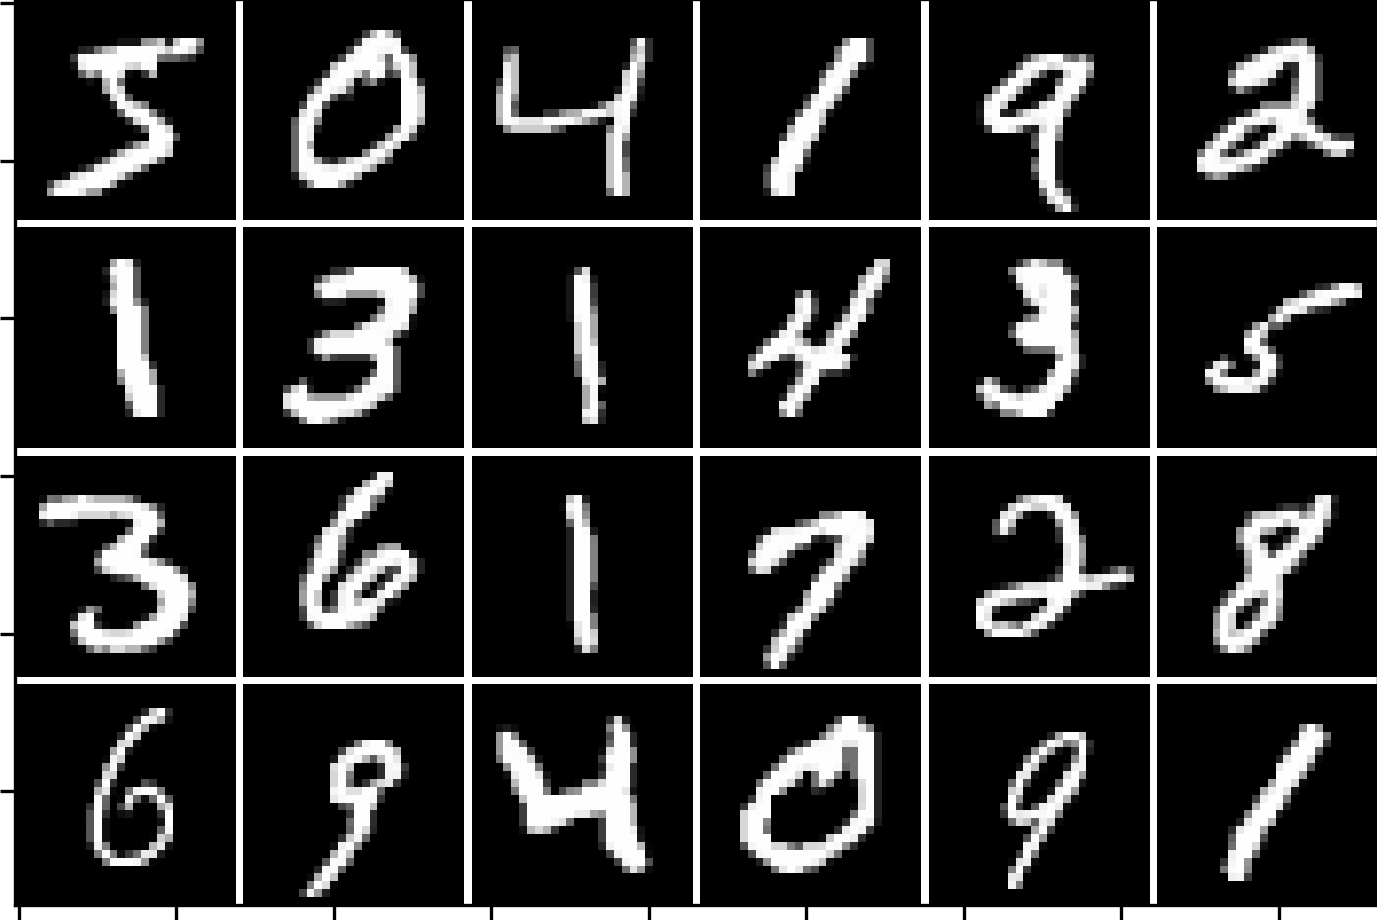
\includegraphics[width=0.7\linewidth]{image/mnist_sample.png}
	\caption{MNISTデータセットの一部}
	\label{fig:mnistsample}
\end{figure}

以下に実験の手順を示す.
先ず,学習データについて畳み込み辞書学習を行い,フィルタを設計及び,学習データの係数マップを得る.本実験では$6$枚の$5\times 5$ピクセルのフィルタを学習させた.
ここで,係数マップのパワースペクトルを特徴として使用する場合は,パワースペクトルを算出後にベクトル化する(係数マップを特徴として用いる場合はそのままベクトル化する).
これらをNMFにより256次元まで次元削減し,それらを特徴ベクトルとする.
各クラスの特徴ベクトルを用いて,錐制約部分空間法及び3層ニューラルネットワーク,SVMを学習させる.

次に,テストデータについて係数を算出する.
具体的には問題(\ref{x-update})を解くのだが,フィルタは学習データで行った畳み込み辞書学習で得られたものを使用する.
また,学習データについてと同様の操作で256次元の特徴ベクトルを得る.
最後に,学習させた各分類器で分類を行い分類精度を算出する.


なお,畳み込み辞書学習の計算にはPythonと,Python用のライブラリSPORCO\cite{sporco}を用いた.

\section{実験結果}
各学習用画像の枚数に対する実験結果を図\ref{result_first}から図\ref{result_last}に示す.
結果より,どの分類器を用いた実験においても,係数のパワースペクトルを特徴として使用すると認識精度が向上することが分かる.
これは画像中の位置ずれを,周波数の使用により吸収したためと考えられる.
また,学習枚数が比較的少ない100枚,200枚,300枚の実験では錐制約部分空間法を用いた場合が最も良い精度であり,データの数が大きくなるにつれてニューラルネットやSVMを用いた方が精度が良くなることがることから,錐制約部分空間法は学習データが少ない状況下で有効な分類器といえる.

\begin{figure}[htbp]
	\begin{minipage}{0.5\hsize}
		\begin{center}
			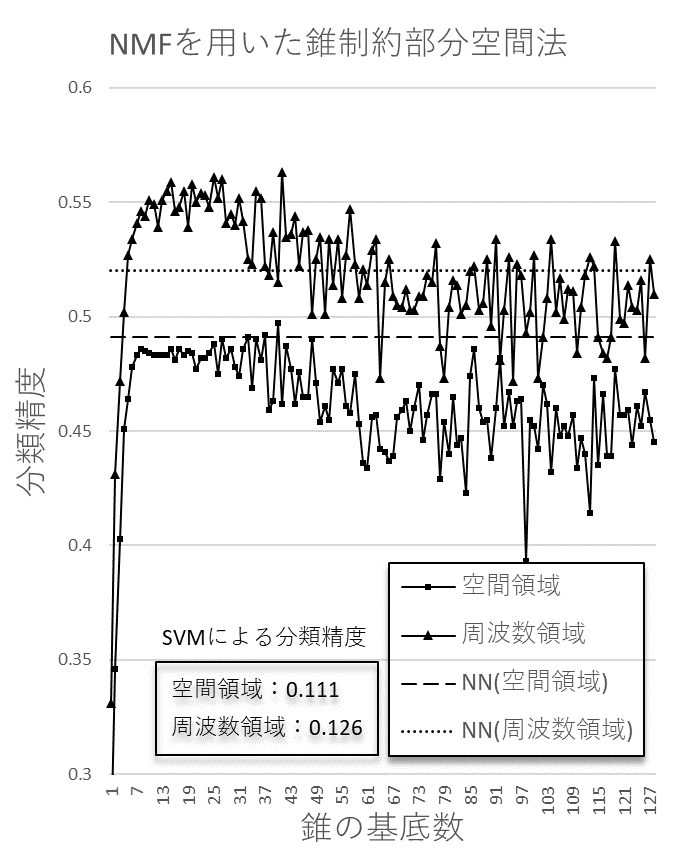
\includegraphics[width=70mm]{result/100-nmf.png}
		\end{center}
		%\caption{一つめの図}
		%\label{fig:one}
	\end{minipage}
	\begin{minipage}{0.5\hsize}
		\begin{center}
			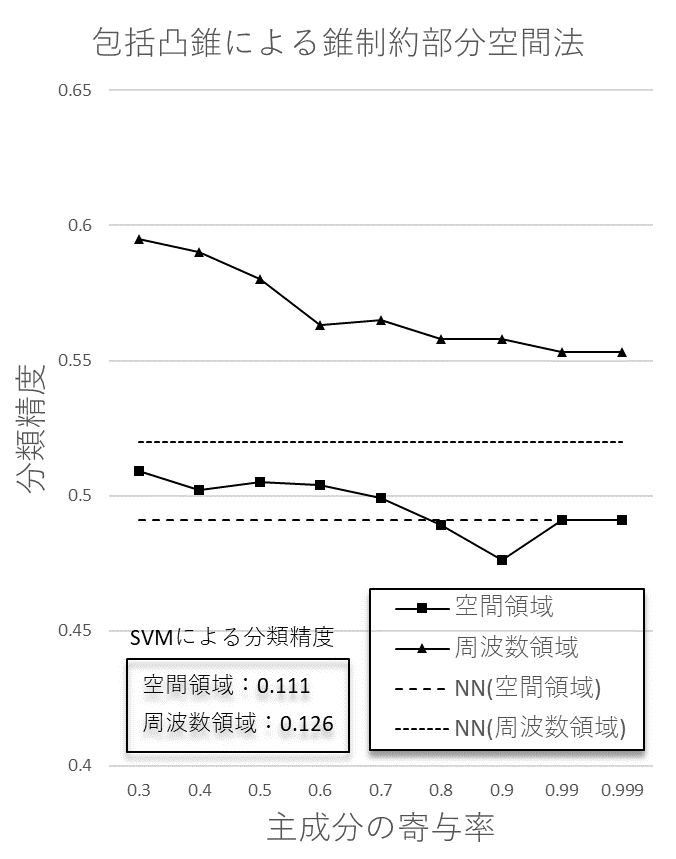
\includegraphics[width=70mm]{result/100-comp.png}
		\end{center}
		%\caption{二つめの図}
		%\label{fig:two}
	\end{minipage}
\caption{学習枚数100枚における分類精度}
\label{result_first}
\end{figure}

\begin{figure}[htbp]
	\begin{minipage}{0.5\hsize}
		\begin{center}
			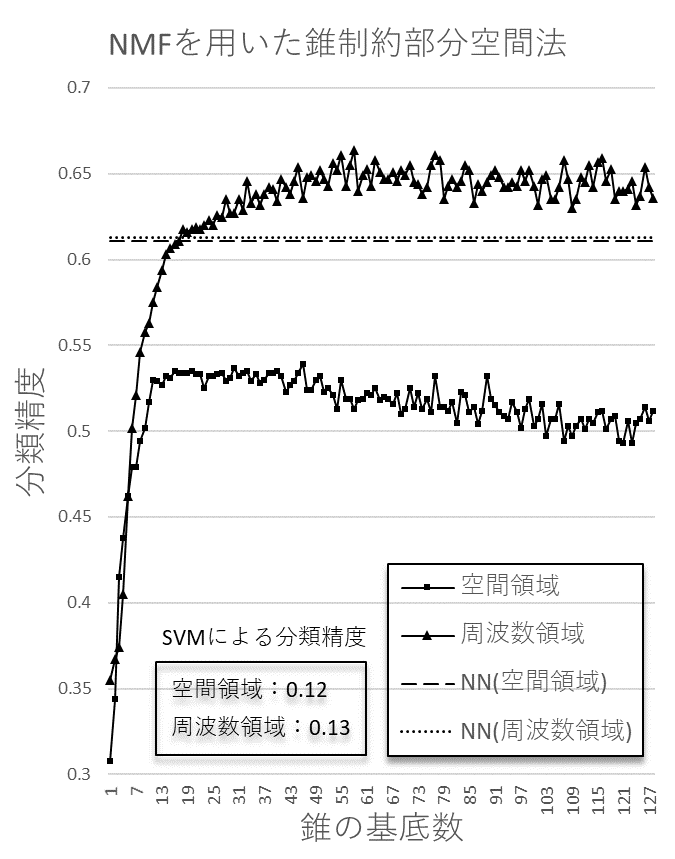
\includegraphics[width=70mm]{result/200-nmf.png}
		\end{center}
		%\caption{一つめの図}
		%\label{fig:one}
	\end{minipage}
	\begin{minipage}{0.5\hsize}
		\begin{center}
			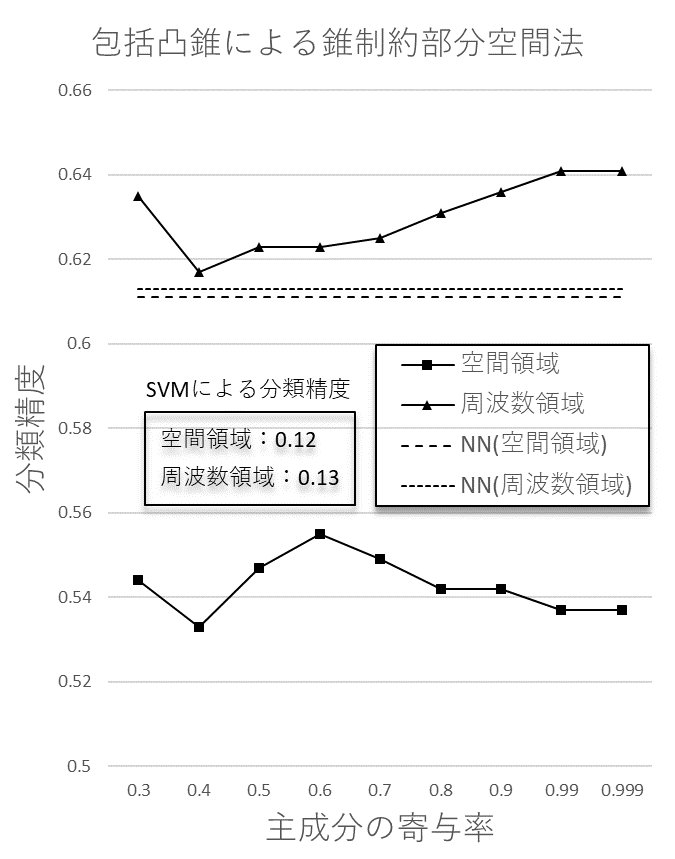
\includegraphics[width=70mm]{result/200-comp.png}
		\end{center}
		%\caption{二つめの図}
		%\label{fig:two}
	\end{minipage}
	\caption{学習枚数200枚における分類精度}
\end{figure}

\begin{figure}[htbp]
	\begin{minipage}{0.5\hsize}
		\begin{center}
			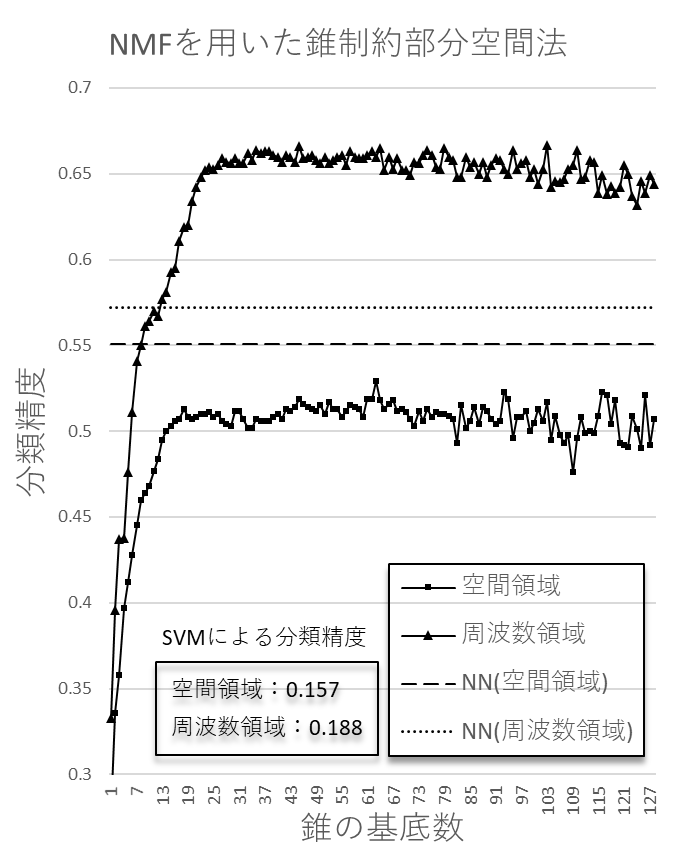
\includegraphics[width=70mm]{result/300-nmf.png}
		\end{center}
		%\caption{一つめの図}
		%\label{fig:one}
	\end{minipage}
	\begin{minipage}{0.5\hsize}
		\begin{center}
			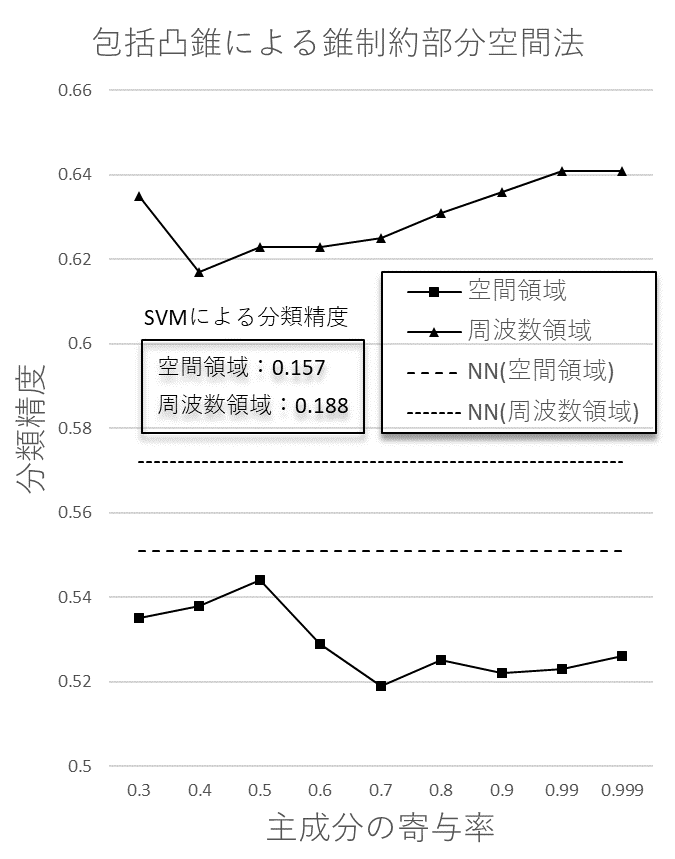
\includegraphics[width=70mm]{result/300-comp.png}
		\end{center}
		%\caption{二つめの図}
		%\label{fig:two}
	\end{minipage}
	\caption{学習枚数300枚における分類精度}
\end{figure}

\begin{figure}[htbp]
	\begin{minipage}{0.5\hsize}
		\begin{center}
			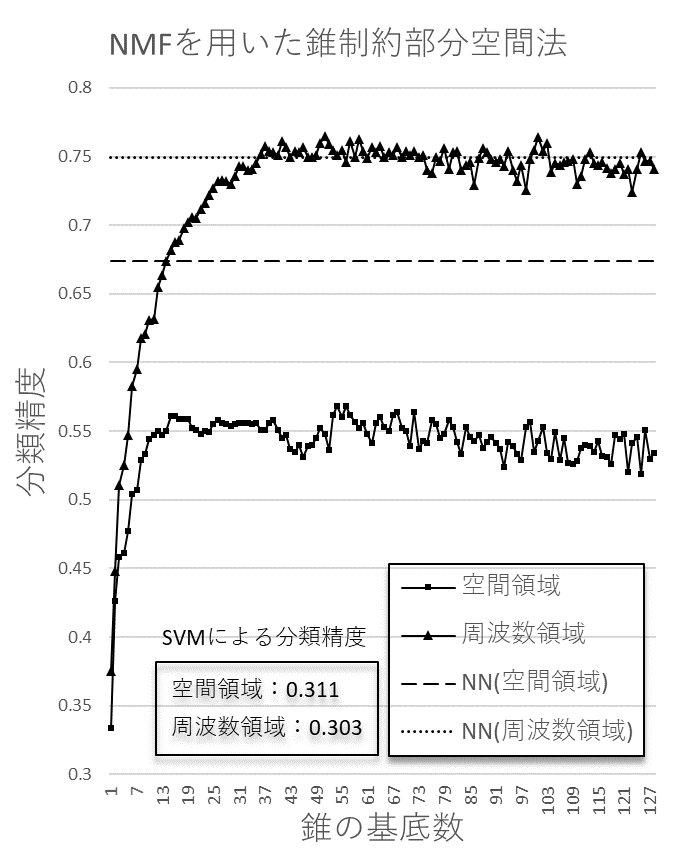
\includegraphics[width=70mm]{result/400-nmf.png}
		\end{center}
		%\caption{一つめの図}
		%\label{fig:one}
	\end{minipage}
	\begin{minipage}{0.5\hsize}
		\begin{center}
			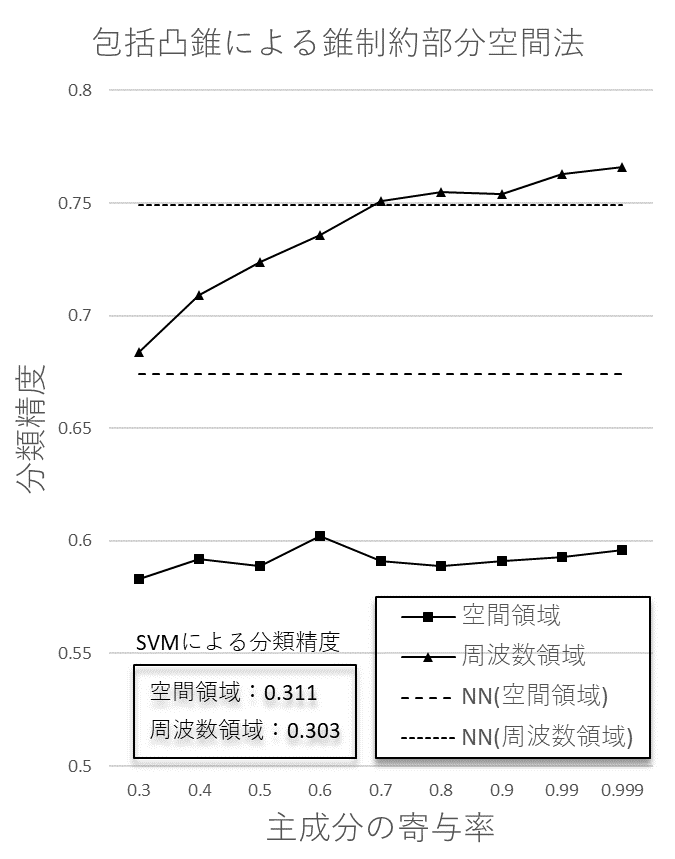
\includegraphics[width=70mm]{result/400-comp.png}
		\end{center}
		%\caption{二つめの図}
		%\label{fig:two}
	\end{minipage}
	\caption{学習枚数400枚における分類精度}
\end{figure}

\begin{figure}[htbp]
	\begin{minipage}{0.5\hsize}
		\begin{center}
			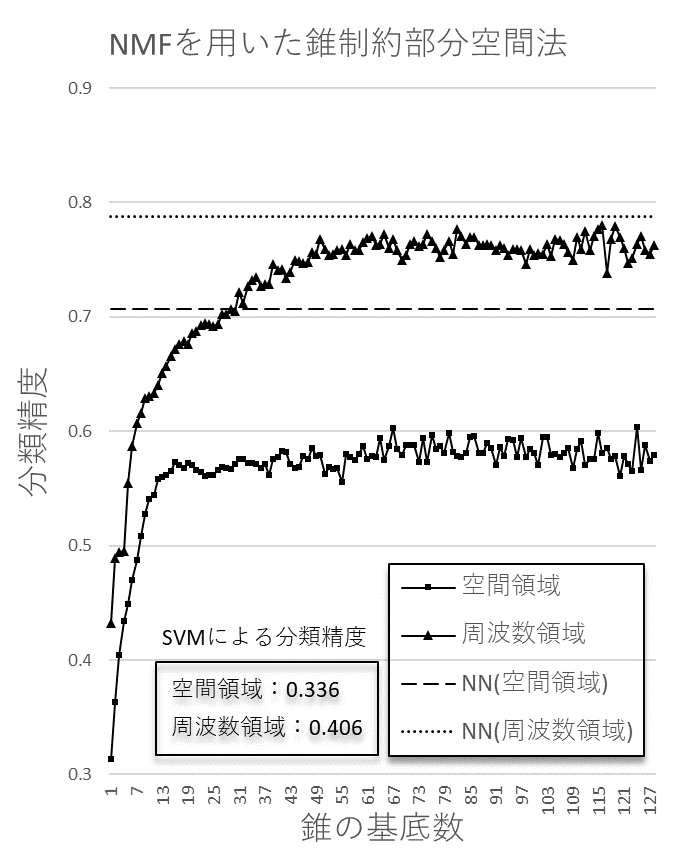
\includegraphics[width=70mm]{result/500-nmf.png}
		\end{center}
		%\caption{一つめの図}
		%\label{fig:one}
	\end{minipage}
	\begin{minipage}{0.5\hsize}
		\begin{center}
			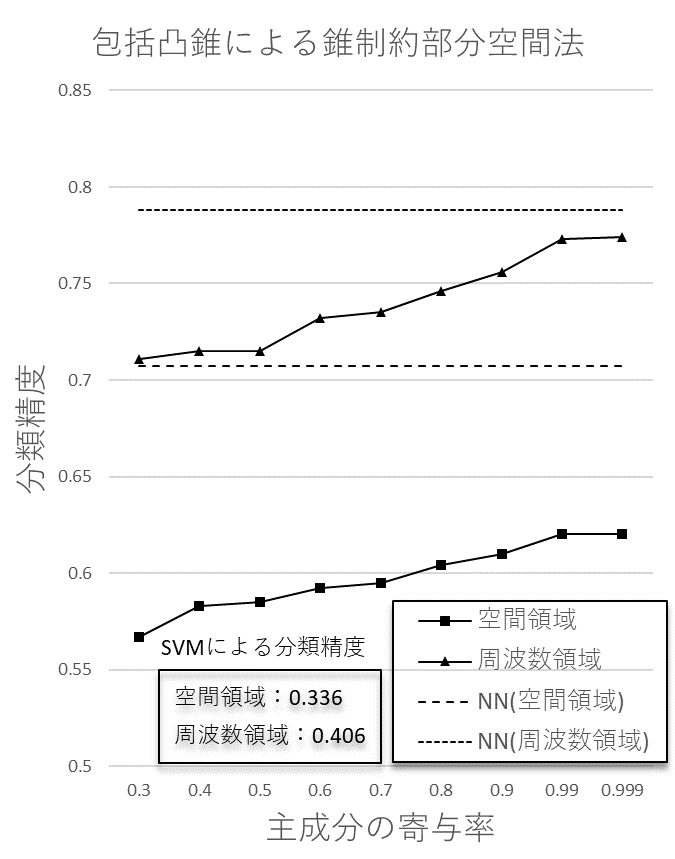
\includegraphics[width=70mm]{result/500-comp.png}
		\end{center}
		%\caption{二つめの図}
		%\label{fig:two}
	\end{minipage}
	\caption{学習枚数500枚における分類精度}
\end{figure}

\begin{figure}[htbp]
	\begin{minipage}{0.5\hsize}
		\begin{center}
			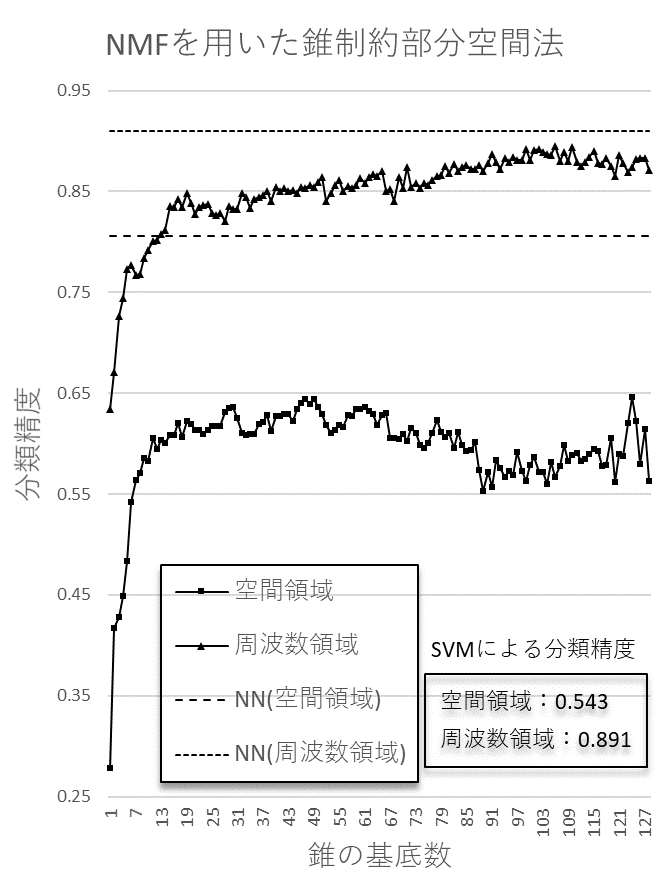
\includegraphics[width=70mm]{result/1000-nmf.png}
		\end{center}
		%\caption{一つめの図}
		%\label{fig:one}
	\end{minipage}
	\begin{minipage}{0.5\hsize}
		\begin{center}
			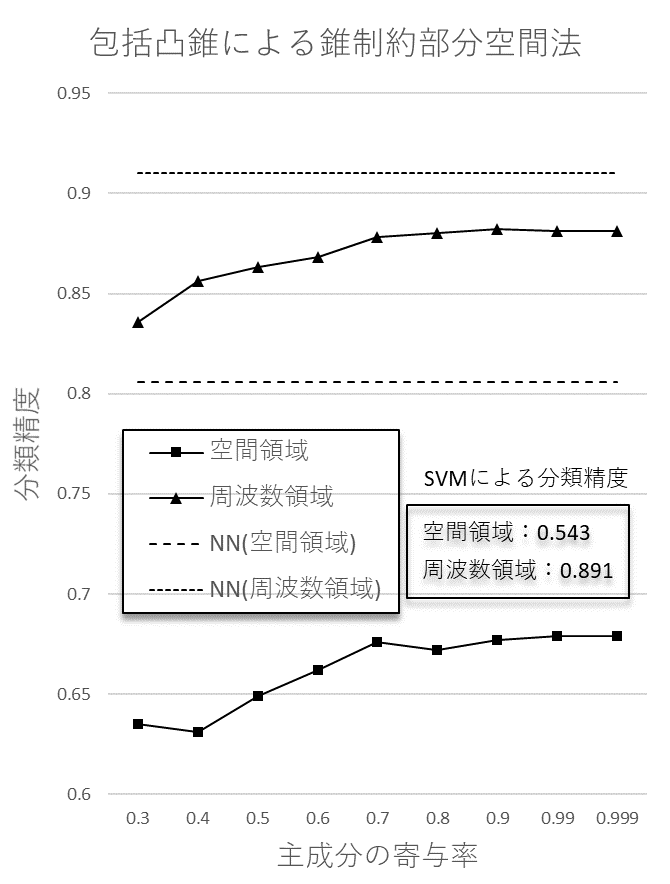
\includegraphics[width=70mm]{result/1000-comp.png}
		\end{center}
		%\caption{二つめの図}
		%\label{fig:two}
	\end{minipage}
	\caption{学習枚数1000枚における分類精度}
	\label{result_last}
\end{figure}


\chapter{むすび}
畳み込み辞書学習における係数マップのパワースペクトルを使用した錐制約部分空間法を提案した.
パワースペクトルの使用は,分類器に依らず精度の向上が確認されたことから,シフト変動に頑健な特徴を示すことが分かった.
また,錐制約部分空間法は他の手法と比較して,学習用データの枚数が少ないときに高い精度を示した.
今後の課題としては,他のデータセットでの評価,多層化された畳み込み辞書学習による係数マップへの適用が考えられる.

\begin{ack}
本研究及びその基礎の学習において,貴重な時間を割いてご指導して頂いた久留米工業高等専門学校制御情報工学科の黒木祥光教授,
および日頃の研究活動において議論を行っていただいた同研究室の専攻科生に深く感謝致します.
\end{ack}


\begin{thebibliography}{9}
\bibitem{fast-csc}
	Bristow, Hilton, Anders Eriksson, and Simon Lucey,”Fast convolutional sparse coding,”Proceedings of the IEEE Conference on Computer Vision and Pattern Recognition. 2013.
	
\bibitem{super-res}
	Gu, Shuhang, et al. ”Convolutional sparse coding for image super-resolution,” Proceedings of the IEEE International Conference on Computer Vision. 2015.

\bibitem{sub}
	福井和広,”部分空間法の今昔 (いまむかし)(下): 最近の技術動向: 相互部分空間法への拡張とその応用事例,” 情報処理 49.6: 680-685,2008.
	
\bibitem{nmf}
	亀岡弘和,”非負値行列因子分解,” 計測と制御 51.9: 835-844,2012.
	
\bibitem{cone-sub}
	小林匠, and 大津展之,”パターン識別のための錐制約部分空間法,” 電子情報通信学会論文誌 D 92.1: 104-111,2009.
	
\bibitem{optimize-csc}
	Bristow, Hilton, and Simon Lucey,”Optimization methods for convolutional sparse coding,” arXiv preprint arXiv:1406.2407 ,2014.
	
\bibitem{admm}
	Boyd, Stephen, et al,”Distributed optimization and statistical learning via the alternating direction method of multipliers,” Foundations and Trends® in Machine learning 3.1: 1-122,2011.
	
\bibitem{sporco}
	Wohlberg, Brendt,”SPORCO: A Python package for standard and convolutional sparse representations,” Proceedings of the 15th Python in Science Conference, Austin, TX, USA. 2017.

\end{thebibliography}

\end{document}
